\documentclass[fleqn]{article}

\usepackage{polski}
\usepackage[utf8]{inputenc}
\usepackage[polish]{babel}
\usepackage{parskip}
\usepackage{icomma}
\usepackage[a4paper,includeheadfoot,margin=1.27cm]{geometry}
\usepackage{float}
\usepackage{graphicx}
\usepackage{amsmath}
\usepackage[hypcap=true]{subcaption}
\usepackage{xcolor}
\usepackage{transparent}
\usepackage{listings}
\usepackage[colorlinks=true, linkcolor=blue, pdfborder={0 0 0}]{hyperref}

\renewcommand\thesection{\arabic{section}.}
\renewcommand\thesubsection{\alph{subsection})}
\renewcommand\thesubsubsection{}
\newcommand\square[1]{
	\fcolorbox{black}{#1}{\rule{0pt}{6pt}\rule{6pt}{0pt}}
}

\brokenpenalty=1000
\clubpenalty=1000
\widowpenalty=1000

\lstdefinestyle{customc}{
	belowcaptionskip=1\baselineskip,
	breaklines=true,
	frame=L,
	xleftmargin=\parindent,
	language=C,
	showstringspaces=false,
	basicstyle=\footnotesize\ttfamily,
	keywordstyle=\bfseries\color{green!40!black},
	commentstyle=\itshape\color{purple!40!black},
	identifierstyle=\color{blue},
	stringstyle=\color{orange},
}


\title{TM -- Laboratorium 6. \\ \large Wskaźnik wysterowania \\ (wartość średnia i maksymalna)}
\author{Krystian Chachuła \\ Dawid Gruszczyński \\ Marcin Skrzypkowski}

\begin{document}

\maketitle

\setcounter{page}{0}
\thispagestyle{empty}

\pagebreak

\setcounter{page}{1}

\section{Cel projektu}

Celem projektu było stworzenie wskaźnika wysterowania, który na wyświetlaczu LCD miał wyświetlać symbole graficzne zależne od poziomu napięcia wejściowego. Miał on prezentować wartość średnią i maksymalną z ustalonej liczby próbek, a tryb wyświetlania miał być przełączany przyciskiem i zachowywany w pamięci nieulotnej.

\section{Założenia i decyzje}

Napięcie mierzone jest przetwornikiem analogowo-cyfrowym, dwunastobitowym, wbudowanym w MSP430. Jego napięciem odniesienia jest poziom 3.3 V. Wynik prezentowany jest na wyświetlaczu LCD 16x2 z podświetleniem, sterowanym przez układ HD77480. W pierwszej jego linii wyświetlamy:
\begin{itemize}
	\item \textbf{tryb pracy}: MAX lub AVG
	\item \textbf{napięcie} w mV zależnie od trybu pracy, średnie lub maksymalne z ustalonej liczby próbek
	\item \textbf{indykator watchdoga}, tzn. jeśli ostatni reset był spowodowany przez WDT, to wyświetlana jest litera W
\end{itemize}
W drugiej linii natomiast znajduje się bargraf wizualizujący napięcie widniejące w pierwszej linii.

Dodatkowo użyliśmy DMA, aby wyniki pomiarów z ADC przekazywać prosto do bufora, który z kolei służył do obliczania wartości średniej oraz maksymalnej napięcia. Układ watchdog został użyty w celu zapobiegnięcia nieprawidłowej pracy urządzenia.

\begin{figure}[H]
	\centering
	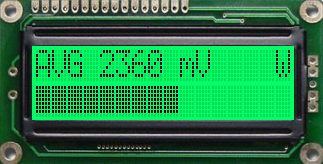
\includegraphics[width=0.75\textwidth]{img/ui.png}
	\caption{Projekt interfejsu użytkownika}
\end{figure}

\pagebreak
\section{Obsługa pamięci flash}
Jednym z głównych założeń projektu było zapisywanie aktualnego trybu wyświetlania w pamięci flash. W naszym przypadku sama dana była stosunkowo prosta, przyjęliśmy wartość $0$ jako oznaczenie trybu wyznaczania średniej arytmetycznej oraz wartość $1$ jako oznaczenie trybu wyświetlania wartości maksymalnej.

Aby umożliwić odnalezienie tych pojedynczych symboli pojedynczą informację zapisywaliśmy na jednym bajcie z ustalonym uprzednio hasłem na siedmiu najbardziej znaczących bitach. Klucz ma wartość $ACh$. Zapis odbywa się do kolejnych bajtów od początku przestrzeni pamięci flash o adresie $01000h$ do $0107Fh$.

Jeśli przekroczona zostanie ilość 128 zapisów, cały segment zostanie wyczyszczony a zapis będzie kontynuowany od początku przestrzeni. Taka implementacja zapisu podyktowana jest sposobem poszukiwania ostatniego zapisu w celu odtworzenia trybu. Poszukujemy danych od ostatnich pozycji w bloku 128 bajtów, pierwszy napotkany bajt z pasującym kluczem jest zarazem ostatnią zapisaną informacją. Kasowanie pamięci jest potrzebne w celu uniknięcia zapętlenia wpisów - wtedy wykrytym trybem byłby zawsze zapisany na bajcie $0107Fh$.

\section{ADC i DMA}
Do mierzenia napięcia wejściowego wykorzystaliśmy przetwornik ADC w trybie repeat-single-channel, który pobudzany zboczem narastającym na wyjściu kanału 1 timera A cyklicznie wykonuje pomiary i wpisuje wyniki do rejestru pamięci ADC12MEM0, skąd do bufora cyklicznego przepisuje je sterownik DMA pracujący w trybie repeated single transfer. Po każdym ustawieniu flagi ADC12IFG następuje transfer do bufora cyklicznego.



\section{Program}
\subsection{main.c}

\begin{minipage}[t]{.49\textwidth}
	\lstinputlisting[lastline=58, style=customc]{../src/main.c}
\end{minipage}\hfill
\noindent\begin{minipage}[t]{.49\textwidth}
	\lstinputlisting[firstline=59, lastline=109, style=customc]{../src/main.c}
\end{minipage}\hfill

\begin{minipage}[t]{.49\textwidth}
	\lstinputlisting[firstline=110, style=customc]{../src/main.c}
\end{minipage}\hfill
\noindent\begin{minipage}[t]{.49\textwidth}
	\subsection{MeasBuffer.h}
	\lstinputlisting[style=customc]{../src/MeasBuffer.h}
	\subsection{MeasBuffer.c}
	\lstinputlisting[style=customc]{../src/MeasBuffer.c}
\end{minipage}\hfill

\end{document}
\grid
